\documentclass{standalone}
\usepackage{tikz}
\usetikzlibrary{arrows.meta, positioning}

\begin{document}

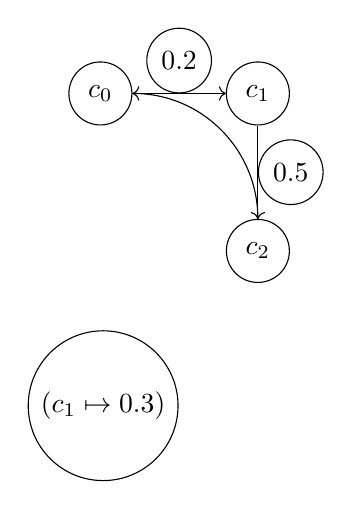
\begin{tikzpicture}[node distance=2cm, every node/.style={circle, draw, minimum size=0.8cm}, every edge/.style={draw, ->, semithick}]
    % Nodes
    \node (c0) {$c_0$};
    \node (c1) [right of=c0] {$c_1$};
    \node (c2) [below of=c1] {$c_2$};

    % Edges
    \draw[->] (c0) to node[above] {0.2} (c1);
    \draw[->] (c1) to node[right] {0.5} (c2);
    \draw[->] (c2) to [bend right=45] (c0);

    % Additional label
    \node[align=center, below left=1cm and 1cm of c2] {$(c_1 \mapsto 0.3)$};

\end{tikzpicture}

\end{document}